\documentclass[11pt]{article}

\usepackage[utf8]{inputenc}
\usepackage{fancyhdr}
\usepackage{hyperref}
\usepackage{graphicx}
\usepackage{amsmath}
\usepackage{amssymb}
\usepackage{natbib}

\graphicspath{ {images/} }
 
\pagestyle{fancy}
\fancyhf{}
\lhead{University of the Witwatersrand}
\rfoot{School of Computer Science and Applied Mathematics}
\pagenumbering{roman}
\fancyfoot[R]{\thepage}
\renewcommand{\headrulewidth}{0pt} % to remove line on header
\renewcommand{\footrulewidth}{0pt} % to remove line on footer

\begin{document}
\begin{page}
\thispagestyle{empty}

\newcommand{\HRule}{\rule{\linewidth}{0.3mm}} % Defines a new command for the horizontal lines, change thickness here
\renewcommand\section{\@startsection{section}{1}{\z@}%
                                  {-3.5ex \@plus -1ex \@minus -.2ex}%
                                  {2.3ex \@plus.2ex}%
                                  {\normalfont\large\bfseries}}
\setlength{\parindent}{0pt}

\center % Center everything on the page
 
%----------------------------------------------------------------------------------------
% HEADING SECTIONS
%----------------------------------------------------------------------------------------

\textsc{\LARGE University of the Witwatersrand}\\[1.5cm] % Name of your university/college
\textsc{\Large School of Computer Science and Applied Mathematics}\\[0.5cm] % Major heading such as course name

%----------------------------------------------------------------------------------------
% TITLE SECTION
%----------------------------------------------------------------------------------------

\HRule \\[0.4cm]
{ \huge \bfseries COMS3008: Parallel Computing Lab Assignment 3}\\[0.4cm] % Title of your document \\
  \large 12 August 2016
\HRule \\[1.5cm]
 
%----------------------------------------------------------------------------------------
% AUTHOR SECTION
%----------------------------------------------------------------------------------------
\begin{minipage}{1\textwidth}
  \Large \emph By Chalom, J. (711985)\\
\end{minipage}


\vfill % Fill the rest of the page with whitespace

\end{page}

\begin{page}
\lfoot{School of Computer Science and Applied Mathematics}
\clearpage
\setcounter{page}{1}
\pagenumbering{arabic}

\section{General Assumptions and Methodology}
All drawn diagrams were drawn using \url{http://draw.io/}, and all results from empirical analysis, were statistically analysed by the data processing program used in lab 1. Those averaged results were then plotted using Microsoft Excel.\\

\noindent The system used for empirical analysis, had an i3 Ivy-bridge CPU, with four processing units and 8GB of RAM. This system can open up a maximum of 26000 threads of computation for a given program excluding any background and operating system tasks.\\

\subsection{Glossary Of Terms:}
\noindent \textbf{\textit{Trapezoid}} - is defined as the British definition (Trapezium) as a quadrilateral with no sides parallel \\
\noindent \textbf{\textit{IBT}} - is an acronym for integration by parts.\\
\noindent \textbf{\textit{STR}} - is an acronym for Simpson's Trapezoidal Rule.\\
\noindent \textbf{\textit{CTR}} - is an acronym for Composite Trapezoidal Rule.\\

\section{Analytical Solution of Given Integral}
\noindent Let $f(x) = \int_{0}^{20} xe^{-x} dx$\\
\\
\noindent By IBT let $\int fdg = fg - \int gdf$, \\
where $f = x$, $dg = e^{-x} dx$, $df = dx$ and $g = -e^{-x}$.\\

\begin{equation} 
\begin{aligned}
    \therefore{} \int xe^{-x} dx = -e^{-x} + \int e^{-x} dx\\ 
\end{aligned}
\end{equation}
\\
\noindent Let $u = -x$ and $dy = -dx$

\begin{equation}
\begin{aligned}
    \therefore{} -e^{-x} + \int e^{-x} dx &= -e^{-x}x - \int e^{u} du\\
    & = -e^{u} - e^{-x}x + c\\
    & = -e^{-x} - e^{-x} + c 
\end{aligned}
\end{equation}
\\

\begin{equation}
\begin{aligned}
    \therefore{} \int_{0}^{20} xe^{-x} dx &= \left[-e^{-x} - e^{-x} + c\right]_{0}^{20} \\
    & = -e^{-20}(20) - e^{-20} + e^{0}(0) + e^{0}\\
    & = 1 - e^{-20}(20) - e^{-20}\\
    & = 1 - \epsilon{}\\
    & \simeq{} 1,00
\end{aligned}
\end{equation}

Note: $\epsilon{} \simeq{} 4,329422607 x 10^{-8}$.
\\
\break
\section{Parallel Trapezoidal Integration}
\subsection{The Trapezium:}
\noindent Let $a$ be the shortest side of a trapezoid (Fig 1), $b$ be the longest side and $h$ be the base of the trapezoid (Fig 1).

\begin{figure}[ht]
\centering
     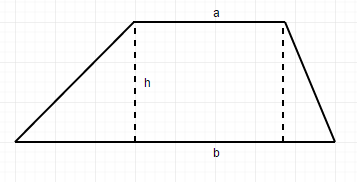
\includegraphics[width=0.40\textwidth]{trapezium}\\
     Fig 1. An example trapezium
\end{figure}

\subsection{The area of a trapezoid is defined as:} 

\begin{equation}
\begin{aligned}
    A &= (a . h) + (\frac{1}{2}(b - a).h)\\
    & = h.(a + \frac{1}{2}(b - a))\\
    & = h.(a + \frac{1}{2}b - \frac{1}{2}a)\\
    & = h.(\frac{1}{2}a + \frac{1}{2}b)\\
    & = \frac{a+b}{2}h
\end{aligned}
\end{equation}
\\
\subsection{Derivation of the rule:}\\
\noindent Let $f(x)$ be a function where $x \in [a,b]$, such that\\
 $a = x_0 < x_1 < ... < x_n = b \in \mathbb{Z}$
 
\begin{figure}[ht]
\centering
     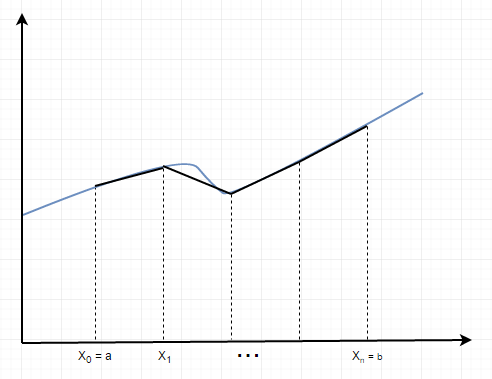
\includegraphics[width=0.80\textwidth]{approx_graph}\\
     Fig 2. Approximation of a polynomial
\end{figure}
\\
\noindent Note: \\
\begin{equation}
\begin{aligned}
    h &= x_{n+1} - x_n\\
    &= \Delta{}x
\end{aligned}
\end{equation}

\noindent The area of the $n^{th}$ trapezoid is given by:\\

\begin{equation}
\begin{aligned}
    A_n = \Delta{x}\Bigg[\frac{f(x_i) + f(x_{i+1})}{2}\Bigg]
\end{aligned}
\end{equation}\\

\noindent Since $\Delta{x}$ is fixed for each partition as it is assumed that there are a uniform number of trapezoids under $f(x)$,\\

\begin{equation}
\begin{aligned}
    \Delta{x} &= \frac{b-a}{n}\\
    \therefore{A_n} &= \Bigg[\frac{f(x_i) + f(x_{i+1})}{2}\Bigg]
\end{aligned}
\end{equation}\\

\noindent Let $m = n-1$, This implies that\\

\begin{equation}
\begin{aligned}
    \int_a^b f(x) dx &\simeq \sum_{i=0}^{m}A_i\\
    &\simeq \sum_{i=0}^{m} \Delta{x} \Bigg[\frac{f(x_i) + f(x_{i+1})}{2}\Bigg]\\
    &\simeq \Delta{x} \sum_{i=0}^{m} \Bigg[\frac{f(x_i) + f(x_{i+1})}{2}\Bigg]\\
    &\simeq \frac{b-a}{2n} \sum_{i=0}^{m} \Bigg[f(x_i) + f(x_{i+1})\Bigg]\\
\end{aligned}
\end{equation}

\subsection{Method of Implementation:}
\noindent The derivation of the Trapezoidal rule (from equation 8) was used and both serial and parallel implementations were programmed. The serial function's results are the baseline for the analysis. The parallel decomposition was a standard openMP parallel for directive where a reduction on the approximation was specified.\\

\noindent The error calculated in these experiments is the result of subtracting the analytical result derived in section 2 by the final approximation at each iteration. If the error is negative then the specific step approximated the integral under the analytical result otherwise it was over the result.\\

\noindent Three result sets were captured. One was the serial implementation where only the main thread was used. This algorithm starts at 1 partition and increments by 100 for 260 iterations. These are the result data points generated.\\

\noindent In the two parallel result sets, one looked at a fixed number of threads (4 threads) and an incrementing number of partitions and the other looked at a fixed number of partitions (1000000) and an incrementing the number of threads from 1 to 26000 threads, at 100 increments 260 times.\\

\noindent All results included the time each specific trapezoidal approximation took to complete, either the number of threads or the number of partitions, the error, and the absolute error.

\subsection{Implementation Results:}\\
\begin{figure}[ht]
\centering
     \includegraphics[width=0.40\textwidth]{}\\
     Fig 1. An example trapezium
\end{figure}

\subsection{Implementation Analysis:}\\

\section{Parallel Monte Carlo Integration}
\subsection{Method of Implementation:}
\noindent A boundary was setup which went from $a = 0$ to $b = 20$ on the $X$ axis and from $c$ to $d$ on the $Y$ axis. $c,d$ are the results of $c = f(a) + 1$ and $d = f(b) + 1$. This produces a rectangle where part of its area is the integral of the function defined in section 2. Random $x$ and $y$ values were generated for every particle in the experiment. They were generated in the range $[a,b]$ and $[c,d]$ respectively. The experiment was conducted using a purely serial function and also a parallel function. The serial function's results are the baseline for the analysis. Each increment taken was repeated 25 times and after the experiment was run averages and other statistics were taken and those results were used to plot the graphs in the results subsection.\\

\noindent The error calculated in these experiments is the result of subtracting the analytical result derived in section 2 by the final approximation at each iteration. If the error is negative then the specific step approximated the integral under the analytical result otherwise it was over the result.\\

\noindent The serial implementation iterated through the number of particles per experiment (from 1 to 26000, at 100 increments) and returned the approximation, an error, the time taken by each calculation and an absolute error.\\

\noindent Both Parallel implementations made used of the same decomposition using openMP's parallel for directive. The private variable for each execution unit was the result of the randomly generated point as the points were never stored in memory for later use. There were shared variables where were $c$ and $d$. A reduction operation was also done on the only variable used outside of the parallel code block, which was variable counting the number of points which occurred below the graph (in side the area of the graph), as the total number of points was known before-hand.\\

\noindent The one parallel experiment locked the number of threads (4 threads) and incremented the number of particles which to generate from 1 particle to 26000 particles incrementing by 100 each time. The other one locked the number of particles at 1000000 and incremented the number of threads from 1 thread to 26000 threads, incrementing by 100 at each step.


\subsection{Implementation Results:}\\
\begin{figure}[ht]
\centering
     \includegraphics[width=0.40\textwidth]{}\\
     Fig 1. An example trapezium
\end{figure}

\subsection{Implementation Analysis:}\\ 

\section{Conclusion}


\break
\section{Appendix A: Alternative Derivation of Trapezoidal Rule}
\subsection{Derivation of the Trapezoidal Rule (STR):}\\
\noindent Let $P_n$ be a polynomial function of n terms.\\

\begin{equation}
\begin{aligned}
    \int_{a}^{b} P_n(x) dx &\simeq{} \int_{a}^{b} f[a]dx + \int_{a}^{b} f[a,b](x-a)dx\\
    &\simeq{} (b-a)f(x) + (\frac{f(b)-f(a)}{(b-a)}).\frac{1}{2}(x-a)^{2}]_{a}^{b}\\
    &\simeq{} (b-a)f(a) + (\frac{f(b)-f(a)}{(b-a)}).\frac{1}{2}(b-a)^{2}\\
    &\simeq{} \frac{b-a}{2}(f(a)+f(b))
\end{aligned}
\end{equation}

\begin{equation}
\begin{aligned}
    Error = \frac{-(b-a)^{3}}{12}f^{''}(\phi)
\end{aligned}
\end{equation} 
\\

\subsection{Derivation of the Composite Trapezoidal Rule (CTR):}\\
\noindent For sub-intervals: $a = x_0 < x_1 < ... < x_n = b$
\\

\begin{equation}
\begin{aligned}
    n &= \frac{b-a}{m}\\
    & = \Delta{x}\\
    & = (x_1 - x_0)
\end{aligned}
\end{equation}
Note: $\Delta{x}$ is fixed.
\\
\begin{equation}
\begin{aligned}
    \int_a^b f(x) dx &= \int_{a=x_0}^{x_1} f(x) + \int_{x_1}^{x_2} f(x) + ... + \int_{x_{n-1}}^{x_n=b} f(x)\\
    &\simeq{} (\frac{x_1 - x_0}{2})[f(x_0) + f(x_1)] + ... + (\frac{x_m - x_{m-1}}{2})[f(x_{m-1}) + f(x_m)]\\
    &\simeq{} \frac{n}{2}[f_0 + 2f_1 + 2f_2 + ... + 2f_{m-1} + f_m]
\end{aligned}
\end{equation}
\\

\begin{equation}
\begin{aligned}
    Error_C_T_R = \frac{(b-a)^3}{12m^2}$ $f^{0}(\phi)$, $\phi \in [a,b]
\end{aligned}
\end{equation}

\end{page}


\end{document}
